\documentclass[12pt,a4paper]{article}

% ─── Page Layout ───────────────────────────────────────────────────────────────
\usepackage[a4paper, margin=0.8in, headheight=14pt]{geometry}

% ─── Fonts (XeLaTeX) ───────────────────────────────────────────────────────────
\usepackage{fontspec}
\usepackage{unicode-math}
\setmainfont{TeX Gyre Pagella}
\setmonofont[Scale=0.88]{TeX Gyre Cursor}
\setmathfont{Latin Modern Math}

% ─── Packages ──────────────────────────────────────────────────────────────────
\usepackage{xcolor}
\usepackage{colortbl}
\usepackage{titlesec}
\usepackage{enumitem}
\usepackage{tabularx}
\usepackage{booktabs}
\usepackage{array}
\usepackage{amsmath}
\usepackage{tikz}
\usetikzlibrary{shapes.geometric, arrows.meta, positioning, calc, fit, decorations.pathreplacing}
\usepackage{tcolorbox}
\tcbuselibrary{skins, breakable}
\usepackage{hyperref}
\usepackage{fancyhdr}
\usepackage{graphicx}
\usepackage{microtype}
\hyphenpenalty=10000
\exhyphenpenalty=10000
\sloppy
\usepackage{caption}
\usepackage{setspace}
\usepackage{multirow}
\usepackage{tocloft}

% ─── Q&A helper ────────────────────────────────────────────────────────────────
\newcommand{\Q}[1]{\textbf{#1}\par\noindent\ignorespaces}

% ─── Colour Palette ────────────────────────────────────────────────────────────
\definecolor{myred}{RGB}{196,30,58}
\definecolor{mydark}{RGB}{30,30,50}
\definecolor{mygreen}{RGB}{14,120,80}
\definecolor{myteal}{RGB}{0,130,140}
\definecolor{myamber}{RGB}{180,100,0}
\definecolor{mypurple}{RGB}{100,30,160}
\definecolor{mygray}{RGB}{246,247,249}
\definecolor{mgframe}{RGB}{180,185,200}
\definecolor{watermark}{RGB}{145,150,170}
\definecolor{hdrred}{RGB}{250,232,235}
\definecolor{hdrgreen}{RGB}{220,244,233}
\definecolor{hdrteal}{RGB}{220,242,244}
\definecolor{hdramber}{RGB}{253,242,215}
\definecolor{hdrpurple}{RGB}{238,228,255}
\definecolor{hdrgray}{RGB}{238,240,245}
\definecolor{rowalt}{RGB}{250,251,253}

% ─── Section Formatting ────────────────────────────────────────────────────────
\titleformat{\section}
  {\large\bfseries\color{myred}}{\thesection.}{0.5em}{}
  [\vspace{1pt}{\color{myred}\rule{\linewidth}{0.8pt}}]
\titleformat{\subsection}
  {\normalsize\bfseries\color{myteal}}{\thesubsection}{0.5em}{}
\titlespacing*{\section}{0pt}{18pt}{7pt}
\titlespacing*{\subsection}{0pt}{11pt}{4pt}

% ─── Paragraph ─────────────────────────────────────────────────────────────────
\setlength{\parindent}{0pt}
\setlength{\parskip}{4pt}

% ─── TOC Styling ───────────────────────────────────────────────────────────────
\renewcommand{\cfttoctitlefont}{\large\bfseries\color{myred}}
\renewcommand{\cftaftertoctitle}{\par\noindent{\color{myred}\rule{\linewidth}{0.8pt}}}
\setlength{\cftbeforetoctitleskip}{0pt}
\setlength{\cftaftertoctitleskip}{6pt}
\renewcommand{\cftsecfont}{\normalsize\bfseries\color{mydark}}
\renewcommand{\cftsecpagefont}{\normalsize\bfseries\color{mydark}}
\renewcommand{\cftsecleader}{\cftdotfill{\cftdotsep}}
\setlength{\cftbeforesecskip}{7pt}
\renewcommand{\cftsubsecfont}{\small\color{mydark}}
\renewcommand{\cftsubsecpagefont}{\small\color{mydark}}
\setlength{\cftbeforesubsecskip}{3pt}
\setlength{\cftsubsecindent}{1.4em}

% ─── Table helpers ─────────────────────────────────────────────────────────────
\renewcommand{\arraystretch}{1.45}
\setlength{\tabcolsep}{6pt}
\arrayrulecolor{mydark}
\newcolumntype{B}[1]{>{\small\bfseries\raggedright\arraybackslash}m{#1}}
\newcolumntype{Y}{>{\small\raggedright\arraybackslash}X}
\renewcommand{\tabularxcolumn}[1]{m{#1}}

% ─── Header / Footer ───────────────────────────────────────────────────────────
\pagestyle{fancy}
\fancyhf{}
\fancyhead[L]{\small\color{myred}\textbf{PE-EC702C}\;\color{mydark}--- Neural Network and Fuzzy Logic Control}
\fancyhead[R]{\small\color{myteal}\textbf{Module 4 Notes}}
\fancyfoot[C]{\small\color{mydark}\thepage}
\fancyfoot[R]{\small\color{watermark}\textit{\copyright\ Biraj}}
\renewcommand{\headrulewidth}{0.5pt}
\renewcommand{\footrulewidth}{0.3pt}

% ─── Hyperref ──────────────────────────────────────────────────────────────────
\hypersetup{
  colorlinks=true, linkcolor=myteal, urlcolor=myteal,
  pdfauthor={Biraj Sarkar},
  pdftitle={PE-EC702C --- Module 4 Notes}
}

% ─── tcolorbox styles ──────────────────────────────────────────────────────────
\tcbset{
  tikzbox/.style={
    colback=mygray, colframe=mgframe, boxrule=0.6pt, arc=4pt,
    left=8pt, right=8pt, top=6pt, bottom=6pt,
    colbacktitle=mgframe, coltitle=mydark,
    fonttitle=\small\bfseries
  },
  defbox/.style={
    colback=hdrgreen, colframe=mygreen, boxrule=0.8pt, arc=4pt,
    left=9pt, right=9pt, top=6pt, bottom=6pt,
    colbacktitle=mygreen, coltitle=white,
    fonttitle=\small\bfseries
  },
  formulabox/.style={
    colback=hdrteal, colframe=myteal, boxrule=0.8pt, arc=4pt,
    left=9pt, right=9pt, top=7pt, bottom=7pt,
    colbacktitle=myteal, coltitle=white,
    fonttitle=\small\bfseries
  },
  examplebox/.style={
    colback=hdramber, colframe=myamber, boxrule=0.8pt, arc=4pt,
    left=9pt, right=9pt, top=6pt, bottom=6pt,
    colbacktitle=myamber, coltitle=white,
    fonttitle=\small\bfseries,
    breakable
  },
  masonbox/.style={
    colback=hdrpurple, colframe=mypurple, boxrule=0.8pt, arc=4pt,
    left=9pt, right=9pt, top=6pt, bottom=6pt,
    colbacktitle=mypurple, coltitle=white,
    fonttitle=\small\bfseries
  },
  exambox/.style={
    colback=hdrpurple, colframe=mypurple, boxrule=1pt, arc=5pt,
    left=10pt, right=10pt, top=8pt, bottom=8pt,
    colbacktitle=mypurple, coltitle=white,
    fonttitle=\bfseries,
    breakable, title after break={\textbf{Frequently Asked / Viva Questions (contd.)}}}
}
\tcbset{breakable}

% ─── TikZ styles ───────────────────────────────────────────────────────────────
\tikzset{
  block/.style={rectangle, draw=myteal, fill=hdrteal,
    text width=2.2cm, align=center, minimum height=0.85cm,
    font=\small, rounded corners=3pt, line width=0.7pt},
  arrow/.style={-Stealth, thick, color=mydark},
  line/.style={thick, color=mydark}
}

% ═══════════════════════════════════════════════════════════════════════════════
\begin{document}
% ═══════════════════════════════════════════════════════════════════════════════

\begin{center}
  {\LARGE\bfseries\color{myred} PE-EC702C --- Neural Network \& Fuzzy Logic Control}\\[5pt]
  {\normalsize\color{mydark} Semester VII \quad$\bullet$\quad 3L:0T:0P \quad$\bullet$\quad 3 Credits}\\[3pt]
  {\normalsize\color{myteal}\textbf{Module 4 Exam Notes: Fuzzy Sets and Membership Functions}}\\[3pt]
  {\small\color{mydark} CGEC \;$|$\; B.Tech ECE (2023--27) \;$|$\; \textit{Biraj Sarkar}}
\end{center}
\vspace{2pt}
\noindent{\color{myred}\rule{\linewidth}{1.5pt}}
\vspace{2pt}

\hypersetup{linkcolor=mydark}
\tableofcontents
\hypersetup{linkcolor=myteal}
\newpage

% ===============================================================================
\section{Classical (Crisp) Sets vs. Fuzzy Sets}
% ===============================================================================

Classical set theory is based on binary logic (true/false, black/white), whereas fuzzy set theory allows for gradual transitions and degrees of membership.

\begin{tcolorbox}[defbox, title={Fuzzy Set}]
A \textbf{Fuzzy Set} $A$ in a universe of discourse $U$ is defined by a membership function $\mu_A(x)$ that maps each element $x \in U$ to a continuous value in the interval $[0, 1]$.
\begin{equation}
  A = \left\{ \left( x, \mu_A(x) \right) \mid x \in U \right\}
\end{equation}
\end{tcolorbox}

\subsection{Standard Fuzzy Operations}
Let $A$ and $B$ be two fuzzy sets with membership functions $\mu_A(x)$ and $\mu_B(x)$ respectively:
\begin{itemize}[leftmargin=*, itemsep=3.5pt]
  \item \textbf{Union (OR / Standard Max):}
    \begin{equation}
      \mu_{A \cup B}(x) = \max\left( \mu_A(x), \mu_B(x) \right) = \mu_A(x) \lor \mu_B(x)
    \end{equation}
  \item \textbf{Intersection (AND / Standard Min):}
    \begin{equation}
      \mu_{A \cap B}(x) = \min\left( \mu_A(x), \mu_B(x) \right) = \mu_A(x) \land \mu_B(x)
    \end{equation}
  \item \textbf{Complement (NOT):}
    \begin{equation}
      \mu_{\bar{A}}(x) = 1 - \mu_A(x)
    \end{equation}
  \item \textbf{Algebraic Product (Dot):} $\mu_{A \cdot B}(x) = \mu_A(x) \cdot \mu_B(x)$
  \item \textbf{Algebraic Sum (Probabilistic sum):} $\mu_{A \hat{+} B}(x) = \mu_A(x) + \mu_B(x) - \mu_A(x)\mu_B(x)$
\end{itemize}

% ===============================================================================
\section{Fuzzy Relations and Composition}
% ===============================================================================

Fuzzy relations map elements from universe $X$ to universe $Y$ with a membership value in $[0, 1]$.

\begin{tcolorbox}[formulabox, title={Fuzzy Compositions}]
Let $R$ be a fuzzy relation from $X$ to $Y$, and $S$ be a fuzzy relation from $Y$ to $Z$.
\par\vspace{4pt}
\textbf{1. Max-Min Composition ($T = R \circ S$):}
\begin{equation}
  \mu_T(x, z) = \max_{y \in Y} \left\{ \min\left( \mu_R(x,y), \mu_S(y,z) \right) \right\}
\end{equation}
\textbf{2. Max-Product Composition ($T = R \bullet S$):}
\begin{equation}
  \mu_T(x, z) = \max_{y \in Y} \left\{ \mu_R(x,y) \cdot \mu_S(y,z) \right\}
\end{equation}
\end{tcolorbox}

\subsection{Tolerance and Equivalence Relations}
Fuzzy relations can possess algebraic properties similar to classical relations:
\begin{itemize}[leftmargin=*, itemsep=3.5pt]
  \item \textbf{Reflexivity:} A relation $R$ on set $X$ is reflexive if the membership of any element paired with itself is 1:
    \begin{equation}
      \mu_R(x, x) = 1 \quad \forall x \in X
    \end{equation}
  \item \textbf{Symmetry:} A relation $R$ is symmetric if order of elements does not affect membership:
    \begin{equation}
      \mu_R(x, y) = \mu_R(y, x) \quad \forall x, y \in X
    \end{equation}
  \item \textbf{Transitivity (Max-Min Transitivity):} A relation $R$ is Max-Min transitive if:
    \begin{equation}
      R \circ R \subseteq R \quad \implies \quad \mu_R(x, z) \ge \max_{y \in X} \left\{ \min\left( \mu_R(x, y), \mu_R(y, z) \right) \right\} \quad \forall x, z \in X
    \end{equation}
\end{itemize}

Based on these properties, we define two special fuzzy relations:
\begin{enumerate}[leftmargin=*, itemsep=3.5pt]
  \item \textbf{Tolerance Relation (Compatibility Relation):} A fuzzy relation that is \textbf{reflexive} and \textbf{symmetric}, but not necessarily transitive. It measures the degree of similarity or compatibility between elements.
  \item \textbf{Equivalence Relation (Similarity Relation):} A fuzzy relation that is \textbf{reflexive}, \textbf{symmetric}, and \textbf{Max-Min transitive}. It generalizes the classical equivalence relation to group elements into fuzzy equivalence classes.
\end{enumerate}

% ===============================================================================
\section{Membership Functions and Standard Forms}
% ===============================================================================

\subsection{Key Geometric Features}
\begin{itemize}[leftmargin=*, itemsep=3pt]
  \item \textbf{Support:} The crisp set containing all elements with non-zero membership: $\{x \in U \mid \mu_A(x) > 0\}$.
  \item \textbf{Core:} The crisp set containing all elements with full membership: $\{x \in U \mid \mu_A(x) = 1\}$.
  \item \textbf{Boundary:} The region with $0 < \mu_A(x) < 1$.
  \item \textbf{Crossover Points:} The elements where membership is exactly $0.5$: $\{x \in U \mid \mu_A(x) = 0.5\}$.
\end{itemize}

\subsection{Standard Shapes}
Standard shapes are used to represent categories like "Warm Temperature" or "High Voltage":

\begin{tcolorbox}[tikzbox, title={Standard Membership Function Shapes}]
\centering
\begin{minipage}{0.48\textwidth}
  \centering
  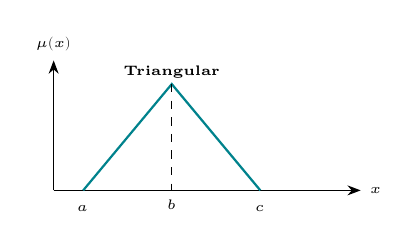
\begin{tikzpicture}[scale=0.75]
    % Axes
    \draw[-Stealth] (0,0) -- (5.2,0) node[right] {\tiny $x$};
    \draw[-Stealth] (0,0) -- (0,2.2) node[above] {\tiny $\mu(x)$};
    % Triangular
    \draw[thick, color=myteal] (0.5,0) -- (2.0,1.8) -- (3.5,0);
    \draw[dashed] (2.0,1.8) -- (2.0,0) node[below] {\tiny $b$};
    \node at (0.5, -0.3) {\tiny $a$};
    \node at (3.5, -0.3) {\tiny $c$};
    \node at (2.0, 2.0) {\textbf{\tiny Triangular}};
  \end{tikzpicture}
\end{minipage}
\hfill
\begin{minipage}{0.48\textwidth}
  \centering
  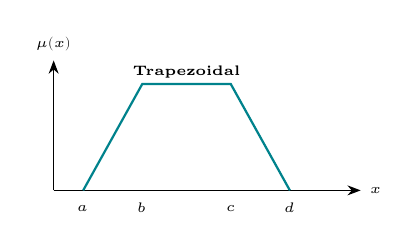
\begin{tikzpicture}[scale=0.75]
    % Axes
    \draw[-Stealth] (0,0) -- (5.2,0) node[right] {\tiny $x$};
    \draw[-Stealth] (0,0) -- (0,2.2) node[above] {\tiny $\mu(x)$};
    % Trapezoidal
    \draw[thick, color=myteal] (0.5,0) -- (1.5,1.8) -- (3.0,1.8) -- (4.0,0);
    \node at (0.5, -0.3) {\tiny $a$};
    \node at (1.5, -0.3) {\tiny $b$};
    \node at (3.0, -0.3) {\tiny $c$};
    \node at (4.0, -0.3) {\tiny $d$};
    \node at (2.25, 2.0) {\textbf{\tiny Trapezoidal}};
  \end{tikzpicture}
\end{minipage}
\end{tcolorbox}

% ===============================================================================
\section{Fuzzification and Defuzzification}
% ===============================================================================

\begin{itemize}[leftmargin=*, itemsep=3pt]
  \item \textbf{Fuzzification:} The process of converting a crisp physical input value into a fuzzy membership value using predefined membership functions.
  \item \textbf{Defuzzification:} The process of converting a combined fuzzy output shape into a single representative crisp output value.
\end{itemize}

\subsection{Standard Defuzzification Methods}
Let $C$ be the output fuzzy set defined on the continuous output space $z$.

\begin{tcolorbox}[formulabox, title={Mathematical Formulations of Defuzzification}]
\textbf{1. Centroid (Center of Gravity - COG):}
\begin{equation}
  z^* = \frac{\int z \mu_C(z) \, dz}{\int \mu_C(z) \, dz} \quad \rightarrow \quad \text{(Discrete: } z^* = \frac{\sum z_i \mu_C(z_i)}{\sum \mu_C(z_i)}\text{)}
\end{equation}
\textbf{2. Mean of Maxima (MOM):}
\begin{equation}
  z^* = \frac{\sum_{z_i \in M} z_i}{|M|} \quad \text{where } M = \{z \mid \mu_C(z) \text{ is maximum}\}
\end{equation}
\textbf{3. First of Maxima (FOM) / Last of Maxima (LOM):}
$z^* = \min(M)$ (First) or $z^* = \max(M)$ (Last).
\end{tcolorbox}

\begin{tcolorbox}[tikzbox, title={Defuzzification Geometric Points}]
\centering
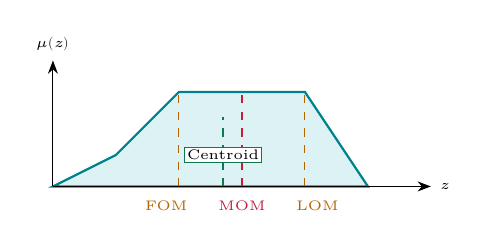
\begin{tikzpicture}[scale=0.8, every node/.style={font=\tiny}]
  % Shape
  \draw[thick, fill=hdrteal, draw=myteal] (0,0) -- (1,0.5) -- (2,1.5) -- (4,1.5) -- (5,0) -- cycle;
  \draw[-Stealth] (0,0) -- (6,0) node[right] {$z$};
  \draw[-Stealth] (0,0) -- (0,2.0) node[above] {$\mu(z)$};

  % MOM
  \draw[dashed, thick, color=myred] (3, 0) -- (3, 1.5);
  \node at (3, -0.3) [color=myred] {MOM};

  % FOM
  \draw[dashed, color=myamber] (2, 0) -- (2, 1.5);
  \node at (1.8, -0.3) [color=myamber] {FOM};

  % LOM
  \draw[dashed, color=myamber] (4, 0) -- (4, 1.5);
  \node at (4.2, -0.3) [color=myamber] {LOM};

  % Centroid
  \draw[dashed, thick, color=mygreen] (2.7, 0) -- (2.7, 1.1);
  \node at (2.7, 0.5) [draw=mygreen, fill=white, inner sep=1pt] {Centroid};
\end{tikzpicture}
\end{tcolorbox}

% ===============================================================================
\section{Lambda Cuts (\texorpdfstring{$\lambda$}{lambda}-cuts)}
% ===============================================================================

A $\lambda$-cut (or $\alpha$-cut) operation converts a fuzzy set or fuzzy relation into a classical (crisp) set by thresholding.

\begin{tcolorbox}[defbox, title={Lambda Cut ($\lambda$-cut)}]
The $\lambda$-cut of a fuzzy set $A$, denoted by $A_{\lambda}$, is a crisp set containing all elements whose membership values are greater than or equal to $\lambda$:
\begin{equation}
  A_{\lambda} = \left\{ x \in U \mid \mu_A(x) \ge \lambda \right\} \quad \text{where } \lambda \in [0, 1]
\end{equation}
\end{tcolorbox}

% ===============================================================================
\section{Worked Examples}
% ===============================================================================

\begin{tcolorbox}[examplebox, title={Fuzzy Set Operations}]
\textbf{Problem:} Given two discrete fuzzy sets defined on $U = \{1, 2, 3, 4\}$:
\begin{equation*}
  A = \left\{ \frac{0.2}{1}, \frac{0.7}{2}, \frac{1.0}{3}, \frac{0.4}{4} \right\}, \quad B = \left\{ \frac{0.5}{1}, \frac{0.6}{2}, \frac{0.3}{3}, \frac{0.9}{4} \right\}
\end{equation*}
Calculate: (a) $A \cup B$, (b) $A \cap B$, and (c) the algebraic product $A \cdot B$.
\par\vspace{4pt}\noindent\rule{\linewidth}{0.5pt}\par
\textbf{Solution:}
Recall: $\mu_{A \cup B} = \max(\mu_A, \mu_B)$, $\mu_{A \cap B} = \min(\mu_A, \mu_B)$, and $\mu_{A \cdot B} = \mu_A \cdot \mu_B$.
\par\vspace{4pt}
\begin{itemize}[leftmargin=*, itemsep=3.5pt]
  \item \textbf{(a) Union ($A \cup B$):}
    \begin{align*}
      \mu_{A \cup B}(1) &= \max(0.2, 0.5) = 0.5 \\
      \mu_{A \cup B}(2) &= \max(0.7, 0.6) = 0.7 \\
      \mu_{A \cup B}(3) &= \max(1.0, 0.3) = 1.0 \\
      \mu_{A \cup B}(4) &= \max(0.4, 0.9) = 0.9 \\
      A \cup B &= \left\{ \frac{0.5}{1}, \frac{0.7}{2}, \frac{1.0}{3}, \frac{0.9}{4} \right\}
    \end{align*}
  \item \textbf{(b) Intersection ($A \cap B$):}
    \begin{align*}
      A \cap B &= \left\{ \frac{\min(0.2,0.5)}{1}, \frac{\min(0.7,0.6)}{2}, \frac{\min(1.0,0.3)}{3}, \frac{\min(0.4,0.9)}{4} \right\} \\
      &= \left\{ \frac{0.2}{1}, \frac{0.6}{2}, \frac{0.3}{3}, \frac{0.4}{4} \right\}
    \end{align*}
  \item \textbf{(c) Algebraic Product ($A \cdot B$):}
    \begin{align*}
      A \cdot B &= \left\{ \frac{0.2 \times 0.5}{1}, \frac{0.7 \times 0.6}{2}, \frac{1.0 \times 0.3}{3}, \frac{0.4 \times 0.9}{4} \right\} \\
      &= \left\{ \frac{0.10}{1}, \frac{0.42}{2}, \frac{0.30}{3}, \frac{0.36}{4} \right\}
    \end{align*}
\end{itemize}
\end{tcolorbox}

\begin{tcolorbox}[examplebox, title={Max-Min Composition of Fuzzy Relations}]
\textbf{Problem:} Given fuzzy relations $R$ (size $2 \times 2$) and $S$ (size $2 \times 2$):
\begin{equation*}
  R = \begin{bmatrix} 0.6 & 0.3 \\ 0.2 & 0.9 \end{bmatrix}, \quad S = \begin{bmatrix} 0.5 & 0.8 \\ 0.7 & 0.1 \end{bmatrix}
\end{equation*}
Compute the Max-Min composition $T = R \circ S$.
\par\vspace{4pt}\noindent\rule{\linewidth}{0.5pt}\par
\textbf{Solution:}
The formulation is $t_{ik} = \max_j \left\{ \min\left(r_{ij}, s_{jk}\right) \right\}$.
\begin{itemize}[leftmargin=*, itemsep=3.5pt]
  \item \textbf{Element $t_{11}$:}
    \begin{equation*}
      t_{11} = \max\left( \min(0.6, 0.5), \min(0.3, 0.7) \right) = \max(0.5, 0.3) = 0.5
    \end{equation*}
  \item \textbf{Element $t_{12}$:}
    \begin{equation*}
      t_{12} = \max\left( \min(0.6, 0.8), \min(0.3, 0.1) \right) = \max(0.6, 0.1) = 0.6
    \end{equation*}
  \item \textbf{Element $t_{21}$:}
    \begin{equation*}
      t_{21} = \max\left( \min(0.2, 0.5), \min(0.9, 0.7) \right) = \max(0.2, 0.7) = 0.7
    \end{equation*}
  \item \textbf{Element $t_{22}$:}
    \begin{equation*}
      t_{22} = \max\left( \min(0.2, 0.8), \min(0.9, 0.1) \right) = \max(0.2, 0.1) = 0.2
    \end{equation*}
\end{itemize}
Thus, the composition is:
\begin{equation*}
  T = R \circ S = \begin{bmatrix} 0.5 & 0.6 \\ 0.7 & 0.2 \end{bmatrix}
\end{equation*}
\end{tcolorbox}

\begin{tcolorbox}[examplebox, title={Discrete Centroid Defuzzification}]
\textbf{Problem:} Calculate the crisp value $z^*$ of the fuzzy set $C$ using Centroid defuzzification:
\begin{equation*}
  C = \left\{ \frac{0.1}{10}, \frac{0.3}{20}, \frac{0.8}{30}, \frac{1.0}{40}, \frac{0.6}{50} \right\}
\end{equation*}
\par\vspace{4pt}\noindent\rule{\linewidth}{0.5pt}\par
\textbf{Solution:}
We use the discrete Centroid formula: $z^* = \frac{\sum z_i \mu_C(z_i)}{\sum \mu_C(z_i)}$.
\par\vspace{4pt}
\begin{align*}
  \sum z_i \mu_C(z_i) &= 10(0.1) + 20(0.3) + 30(0.8) + 40(1.0) + 50(0.6) \\
  &= 1 + 6 + 24 + 40 + 30 = 101 \\
  \sum \mu_C(z_i) &= 0.1 + 0.3 + 0.8 + 1.0 + 0.6 = 2.8 \\
  z^* &= \frac{101}{2.8} \approx 36.07
\end{align*}
The defuzzified crisp output is $z^* \approx 36.07$.
\end{tcolorbox}

\newpage

% ===============================================================================
% MANDATORY QUICK REVISION PAGE
% ===============================================================================
\begin{center}
  {\large\bfseries\color{myred} Quick Revision --- Module IV}\\[3pt]
  {\small\color{mydark} Fuzzy Sets and Membership Functions $|$ PE-EC702C}
\end{center}
\noindent{\color{myred}\rule{\linewidth}{1.2pt}}
\vspace{4pt}

\begin{tcolorbox}[formulabox, title={\textbf{Key Formulas at a Glance}}]
\renewcommand{\arraystretch}{1.3}
\begin{tabularx}{\linewidth}{B{5.0cm} X}
Fuzzy Union (OR) & $\mu_{A \cup B}(x) = \max(\mu_A(x), \mu_B(x))$ \\
Fuzzy Intersection (AND) & $\mu_{A \cap B}(x) = \min(\mu_A(x), \mu_B(x))$ \\
Max-Min Composition & $\mu_{R \circ S}(x, z) = \max_y \{ \min( \mu_R(x,y), \mu_S(y,z) ) \}$ \\
Max-Product Composition & $\mu_{R \bullet S}(x, z) = \max_y \{ \mu_R(x,y) \cdot \mu_S(y,z) \}$ \\
Centroid Defuzzification & $z^* = \frac{\sum z_i \mu_C(z_i)}{\sum \mu_C(z_i)} \quad \text{or} \quad \frac{\int z \mu_C(z) dz}{\int \mu_C(z) dz}$ \\
Lambda-Cut ($\lambda$-cut) & $A_{\lambda} = \{ x \in U \mid \mu_A(x) \ge \lambda \}$
\end{tabularx}
\tcbset{colbacktitle=myteal, coltitle=white}
\end{tcolorbox}

\begin{tcolorbox}[defbox, title={\textbf{One-Line Definitions}}]
\begin{itemize}[leftmargin=*, itemsep=2.5pt, topsep=0pt]
  \item \textbf{Fuzzy Set:} A set containing elements with varying degrees of membership represented by values in $[0, 1]$.
  \item \textbf{Membership Function:} The graphical curve or mathematical function that maps elements to their membership degrees.
  \item \textbf{Centroid Defuzzification:} A defuzzification method that calculates the center of gravity of the output fuzzy region.
  \item \textbf{Lambda Cut:} An operation that converts a fuzzy set/relation into a classical set using a threshold value $\lambda$.
  \item \textbf{Crossover Point:} Any element in the universe of discourse whose membership degree in a fuzzy set is exactly $0.5$.
\end{itemize}
\tcbset{colbacktitle=myteal, coltitle=white}
\end{tcolorbox}

\begin{tcolorbox}[exambox, title={\textbf{Frequently Asked / Viva Questions}}]
\begin{enumerate}[leftmargin=*, itemsep=3.5pt, label=\arabic*.]
  \item \Q{What is the difference between probability and fuzziness?} Probability deals with the likelihood/chance of an event occurring (undecided outcome). Fuzziness deals with the vagueness of an event that has already occurred (deterministic but vague boundaries, e.g. "He is tall").
  \item \Q{State the properties of classical sets that do NOT hold in fuzzy sets.} The Law of Contradiction ($A \cap \bar{A} = \emptyset$) and the Law of Excluded Middle ($A \cup \bar{A} = U$) do not hold in fuzzy sets (e.g. $A \cap \bar{A} \neq \emptyset$).
  \item \Q{What is a normal fuzzy set?} A fuzzy set is normal if its height is exactly $1.0$ (i.e. at least one element has a membership value of $1$).
  \item \Q{Define a subnormal fuzzy set.} A fuzzy set whose maximum membership value (height) is strictly less than $1.0$.
  \item \Q{Why is Centroid defuzzification the most commonly used method?} Because it integrates the entire area of the output fuzzy shape, yielding smooth, continuous output transitions relative to changes in inputs.
  \item \Q{Explain the Max-Min composition rule.} It is a method of relating elements of set $X$ to set $Z$ through intermediate set $Y$. For each $(x,z)$ pair, it finds the strength of paths through all $y \in Y$ (using Min) and selects the strongest path (using Max).
  \item \Q{What is the difference between a tolerance relation and an equivalence relation?} An equivalence relation must be reflexive, symmetric, and transitive. A tolerance relation is only reflexive and symmetric (not transitive).
  \item \Q{Define the support of a fuzzy set.} The crisp set of all elements in the universe of discourse whose membership values are strictly greater than $0$ ($\mu_A(x) > 0$).
  \item \Q{What are the standard forms of membership functions?} Triangular, Trapezoidal, Gaussian, Sigmoidal, L-shaped, and S-shaped curves.
  \item \Q{What is the purpose of defuzzification in fuzzy controllers?} Physical actuators and microcontrollers require crisp, exact values (like voltage or valve position) to operate, which requires defuzzification of the fuzzy control decision.
\end{enumerate}
\tcbset{colbacktitle=myteal, coltitle=white}
\end{tcolorbox}

\begin{tcolorbox}[tikzbox, title={Crisp Sets vs. Fuzzy Sets}]
\centering
\renewcommand{\arraystretch}{1.2}
\begin{tabularx}{\linewidth}{>{\bfseries}B{3.2cm} Y Y}
Attribute & Classical (Crisp) Sets & Fuzzy Sets \\
\midrule
Membership Values & Binary: $\{0, 1\}$ & Continuous: $[0, 1]$ \\
Boundaries & Sharp, distinct boundaries & Gradual, vague boundaries \\
Operations & Boolean logic (AND, OR, NOT) & Fuzzy logic (Min, Max, $1-\mu$) \\
Contradiction Law & Holds: $A \cap \bar{A} = \emptyset$ & Does not hold: $A \cap \bar{A} \neq \emptyset$ \\
\bottomrule
\end{tabularx}
\tcbset{colbacktitle=myteal, coltitle=white}
\end{tcolorbox}

\end{document}
